%%%%%%%%%%%%%%%%%%%%%%%%%%%%%%%%%%%%%%%%%%%%%%%%%%%%%%%%%%%%%%%%%%%%
% Proof Of Concept
%%%%%%%%%%%%%%%%%%%%%%%%%%%%%%%%%%%%%%%%%%%%%%%%%%%%%%%%%%%%%%%%%%%%

\chapter{Proof of concept}
  \label{POC}
  
This chapter describes the experiments that were done with this tool in an attempt to validate a proof sketch proposed by Yannakakis \cite{yannakakis1986four} in 1986.
\section{Idea}
As mentioned in \autoref{PR}, Yannakakis proved in 1986 that all planar graphs can be embedded in books with at most four stacks \cite{yannakakis1986four, yannakakis1989embedding}. Yet to this day there is no planar graph proposed in the literature that needs four stacks, thus the question remains whether there exists a graph that genuinely requires four stacks.  \\
Yannakakis sketched a proof (see \cite{yannakakis1986four}) that utilizes three different graphs which in combination would yield a graph with book thickness four. This sketch appeared in an extended abstract of a paper but it was not finalized in the subsequent journal version of it \cite{yannakakis1989embedding}.\\
This sketch provides motivation for the framework of this thesis. The description of the three graphs are to the best of our understanding and described in the following.

\subsection{Step 1}
\label{S1}
The first graph described by Yannakakis is composed of a path $p = x_0, x_1, ..., x_n$, where $n$ should be sufficiently big (e.g. $n = 1000$). Then add two vertices $A$ and $B$, and connect them to each $x_i$ of the path (see \autoref{YannakakisGraphs}).\\
It seems that the property of this graph is that with a large enough $n$ in any 3-stack linear layout of this graph several consecutive pairs of vertices from path $p$, say $\langle y_1, y_2 \rangle ... \langle y_{2k-1}, y_{2k} \rangle$ lie in the same interval from $A$ to $B$ on the spine. 
This property is important in order to resume to the second step.

\subsection{Step 2}
\label{S2}
The second graph is an augmentation of the first, where each of its inner triangular faces is stellated, that is to say one vertex is added in the center and connected to each of its vertices. Let $a_i$ be the vertex that is added to the face $\langle y_i, y_{i+1}, A\rangle$ and $b_i$ the new vertex in the face $\langle y_i, y_{i+1}, B \rangle$.\\
To the best of our understanding, the property of this graph is that if $k$ is sufficiently large, then in any linear layout there exist four vertices $\langle y_{2_{}0-1}, a_{i_0}, b_{i_0}, y_{2i_0} \rangle$ that appear in this order between $A$ and $B$. 

\subsection{Step 3}
\label{S3}
In the third step, the graph of step 2 gets further augmented. Central in this step is a planar graph $Q$, whose outer face is delimited by a path $(s,a,t,b)$. This graph $Q$ is not fully defined in the proof sketch but should be constructed in a way that it does not admit a 3-stack layout in which 
\begin{enumerate}
\item[a)] the partial order of its four vertices is either $(s,a,b,t)$ or $(s,b,a,t)$ or any of the corresponding cyclic rotations and
\item[b)] the edges incident to $s$ and $t$, which connect to vertices that lie in the interval from $s$ to $t$ on the spine of the linear layout, cannot be assigned to the third stack.
\end{enumerate}
Three copies of this graph $Q$ are attached to each edge $(u,v)$ of the graph from step 2 such that the vertices $s$ and $t$ of graph $Q$ are identified with vertices $u,v$.
\begin{figure}[h!]
\begin{center}
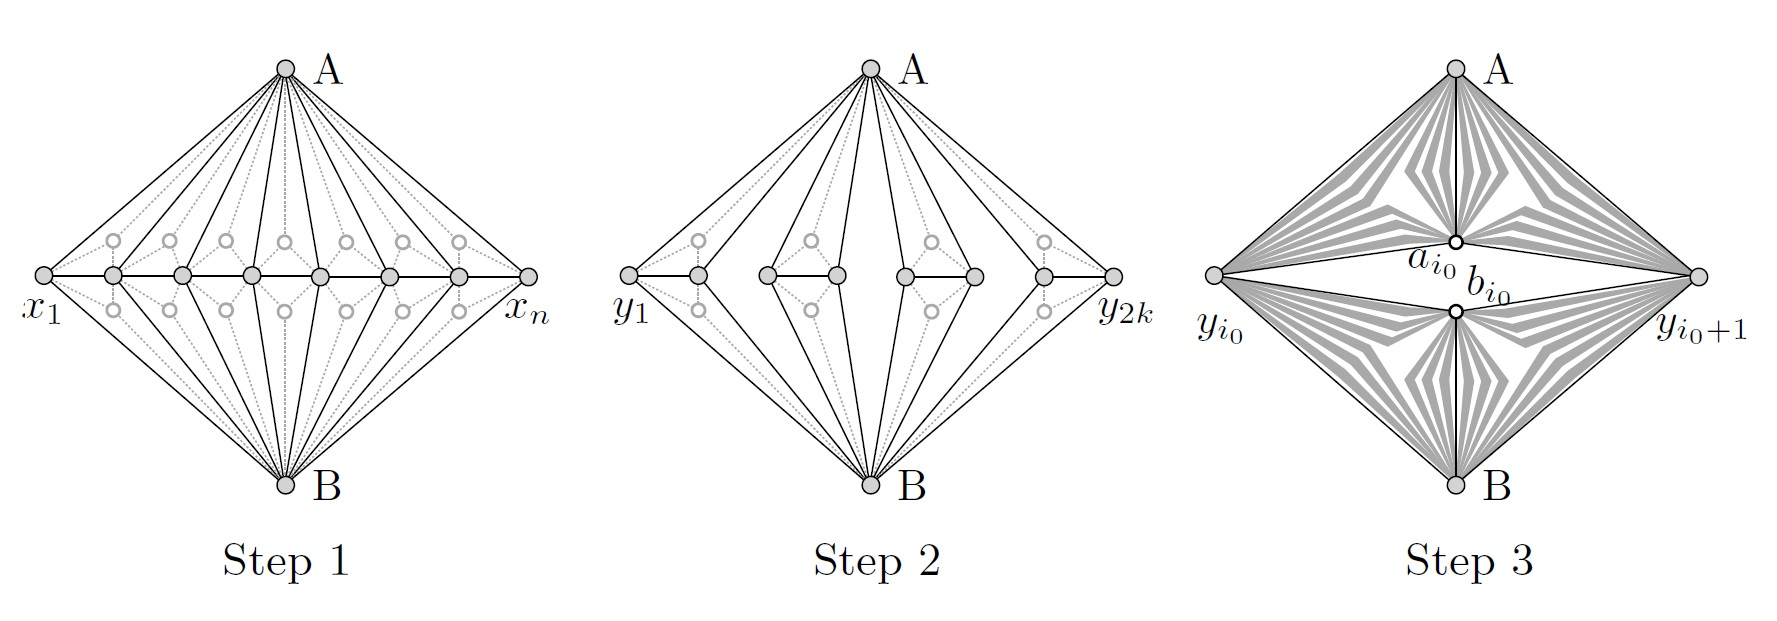
\includegraphics[width=1\textwidth]{figures/yannakakis.jpg}
\caption{Schematic drawings of the constructed graph through all three steps; source: \cite{bekos2019}}
\label{YannakakisGraphs}
\end{center}
\end{figure}
\section{Our findings}
First, we constructed an instance of the graph described in \autoref{S1} with $n=100$ and imposed the following constraints: vertex $A$ should be a predecessor of every vertex $x_{2i-1}$ and successor of every vertex $x_{2i}$, while vertex $B$ should be a successor of every $x_{2i-1}$ and predecessor of every $x_{2i}$. This was done using the \textit{predecessor} constraint described in \autoref{linRestr}.\\
We observed that a linear layout under these constraints exists and we were further able to extend the obtained solution to any $n$.\\
For step 2, we assumed that somehow several pairs of consecutive vertices $\langle y_1, y_2 \rangle ... \langle y_{2k-1}, y_{2k} \rangle$ from path $p$ appear between $A$ and $B$. So next we forbid the partial orders $\langle y_{2i-1}, a_i, b_i, y_{2i} \rangle$ and $\langle y_{2i-1}, b_i, a_i, y_{2i} \rangle$ and asked whether a 3-page book embedding exists under these additional constraints (see also the \textit{restrict partial order} constraint described in \autoref{linRestr}). Again we observed that a linear layout under these constraints exists and we were further able to extend the obtained solution to any $n$.\\
We conclude this section by mentioning that we were not able to find a graph with the properties of graph $Q$ described in \autoref{S3} (see \autoref{linRestr}, \textit{Assign edges incident to certain vertices}).

\begin{figure}[h!]
\begin{center}
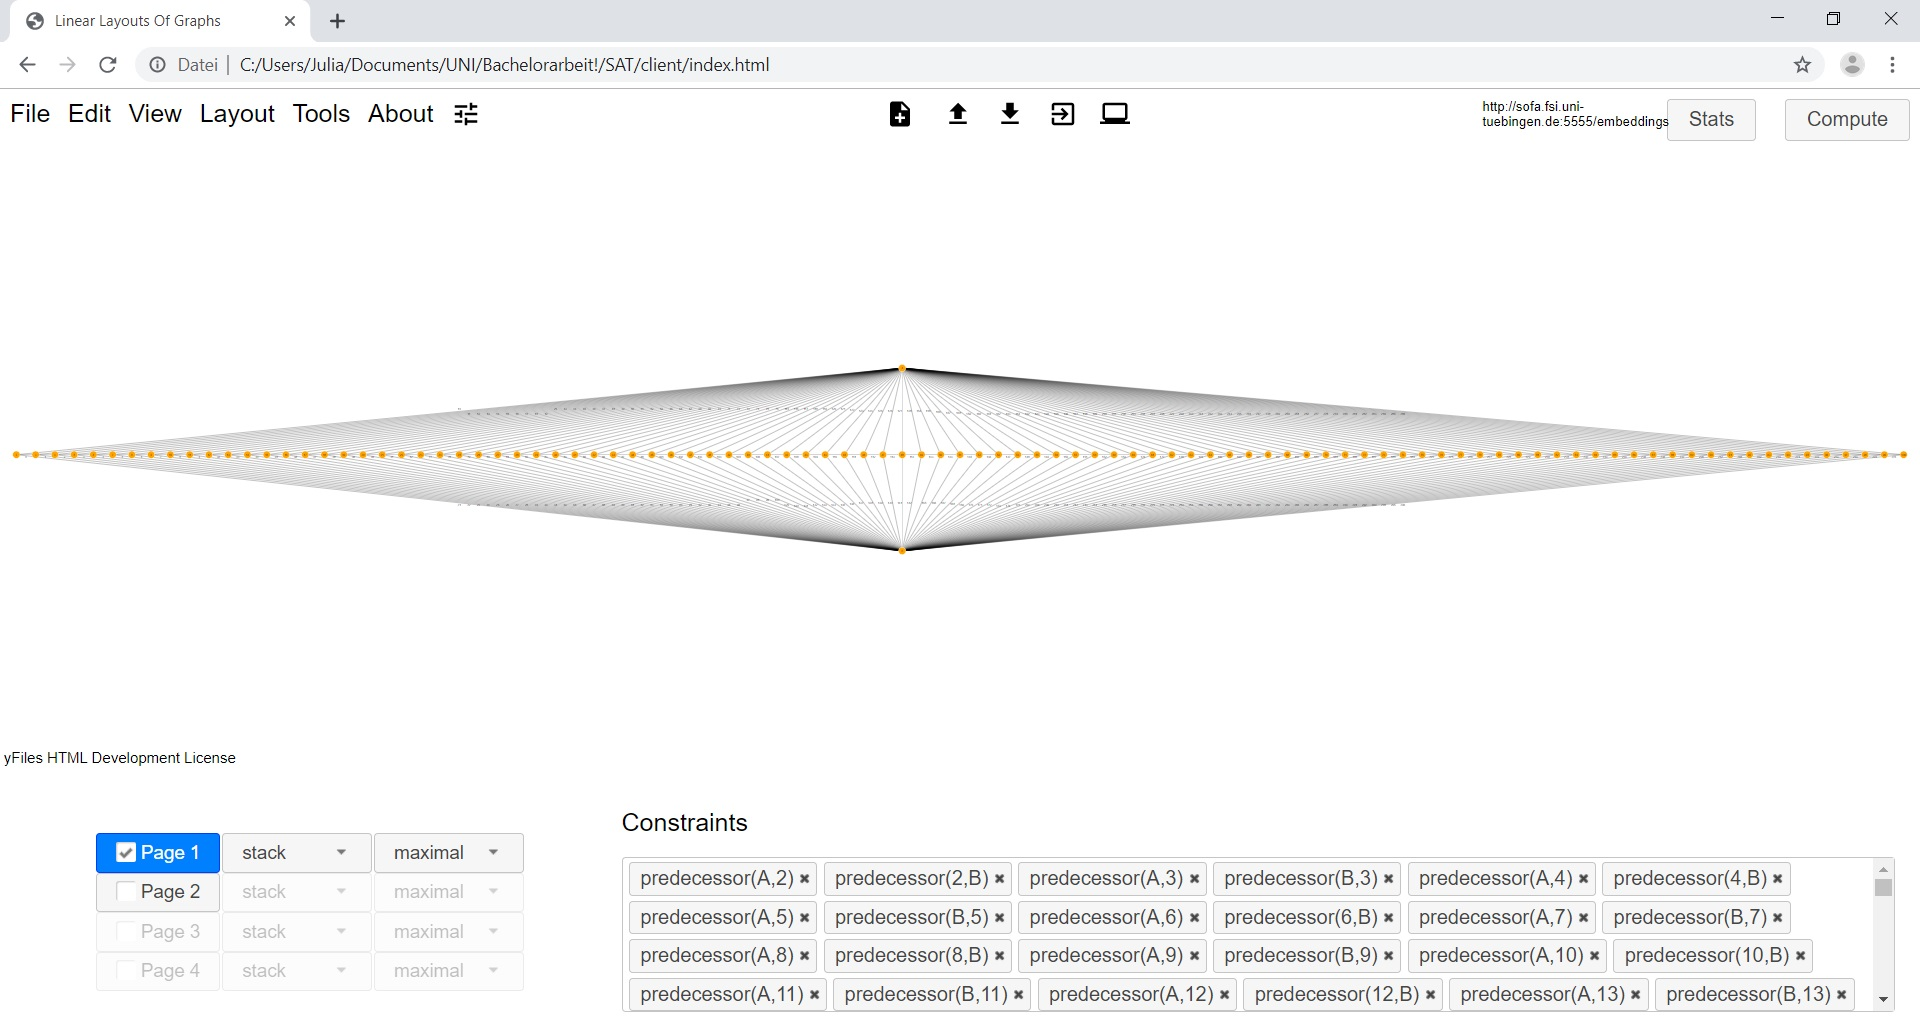
\includegraphics[width=1\textwidth]{figures/skeletonGraph101-296.jpg}
\caption{Our interpretation of the first graph, with 101 vertices and 296 edges as described in \autoref{S1}\label{s1graph}}
\end{center}
\end{figure}
\begin{figure}[h!]
\begin{center}
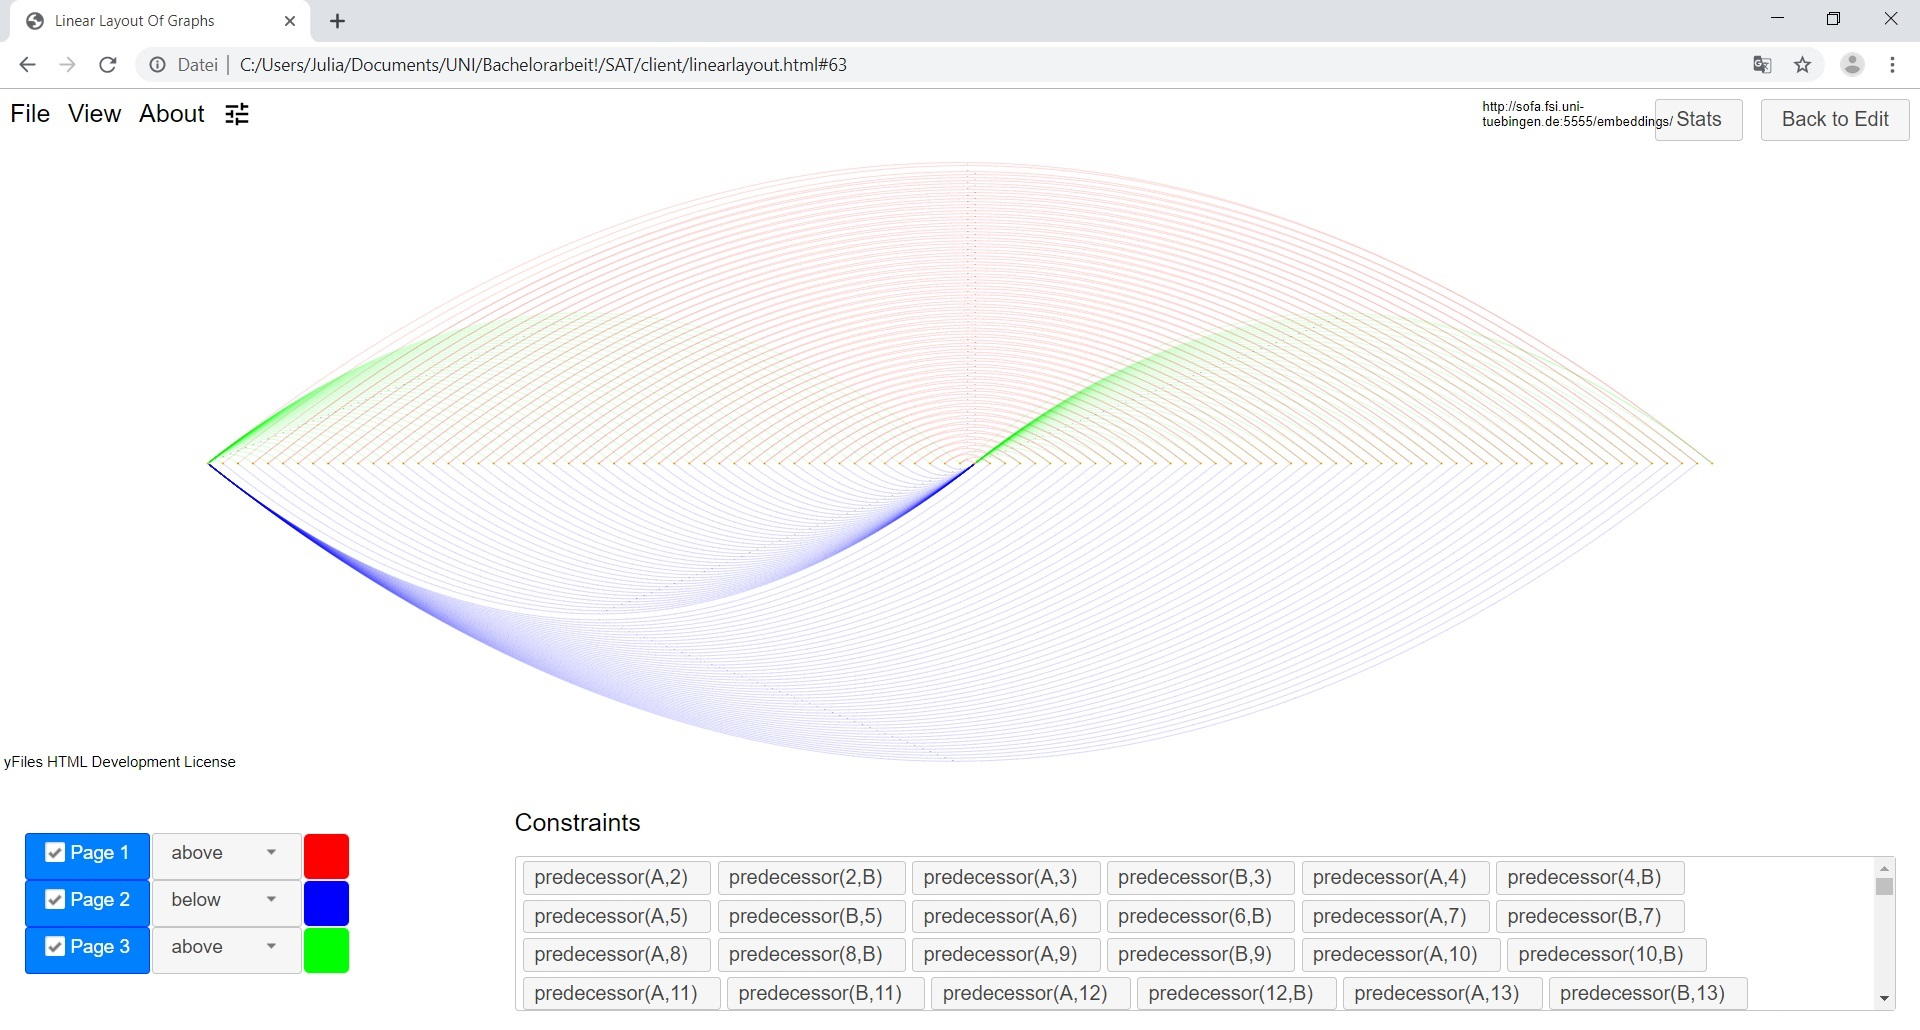
\includegraphics[width=1\textwidth]{figures/skeletonGraph101-296-Solution.jpg}
\caption{The corresponding linear layout to graph in \autoref{s1graph}\label{s1sol}}
\end{center}
\end{figure}

\begin{figure}[h!]
\begin{center}
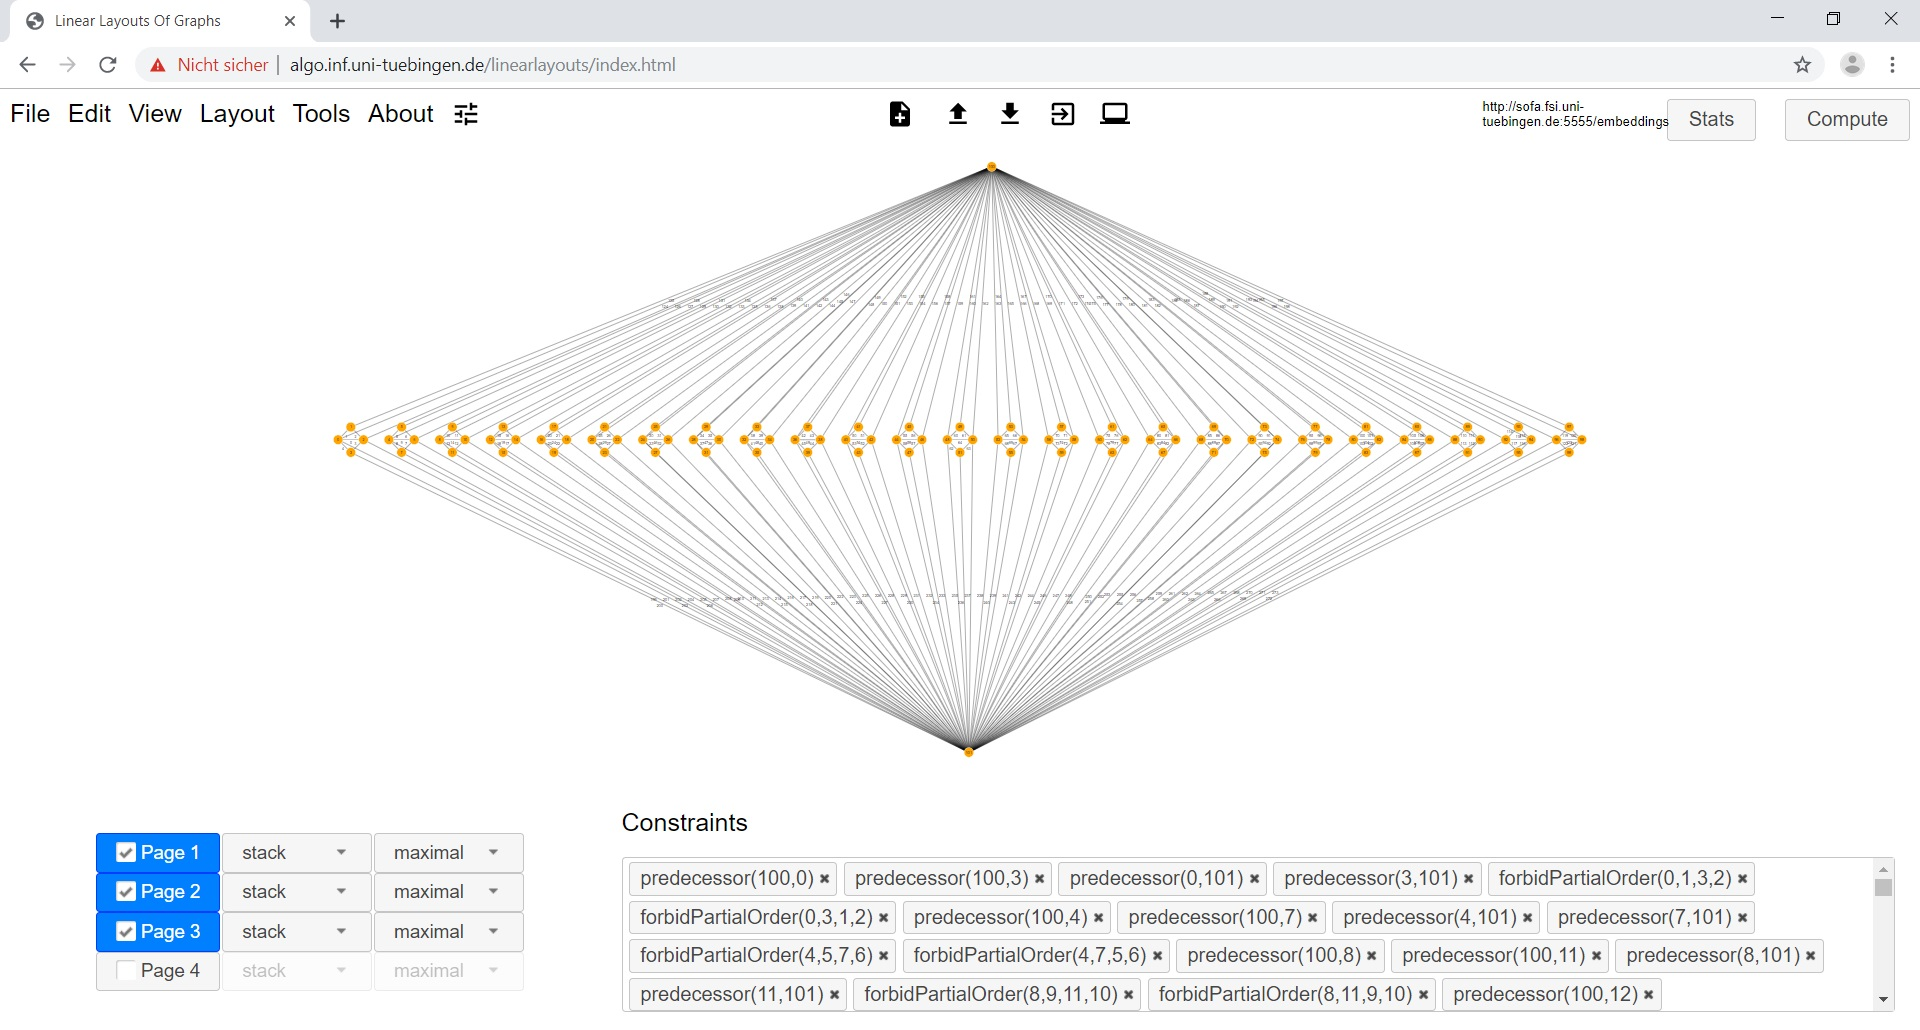
\includegraphics[width=1\textwidth]{figures/stellated-102-274.jpg}
\caption{Our interpretation of the second graph, with 102 vertices and 274 edges as described in \autoref{S2} \label{s2graph}}
\end{center}
\end{figure}
\begin{figure}[h!]
\begin{center}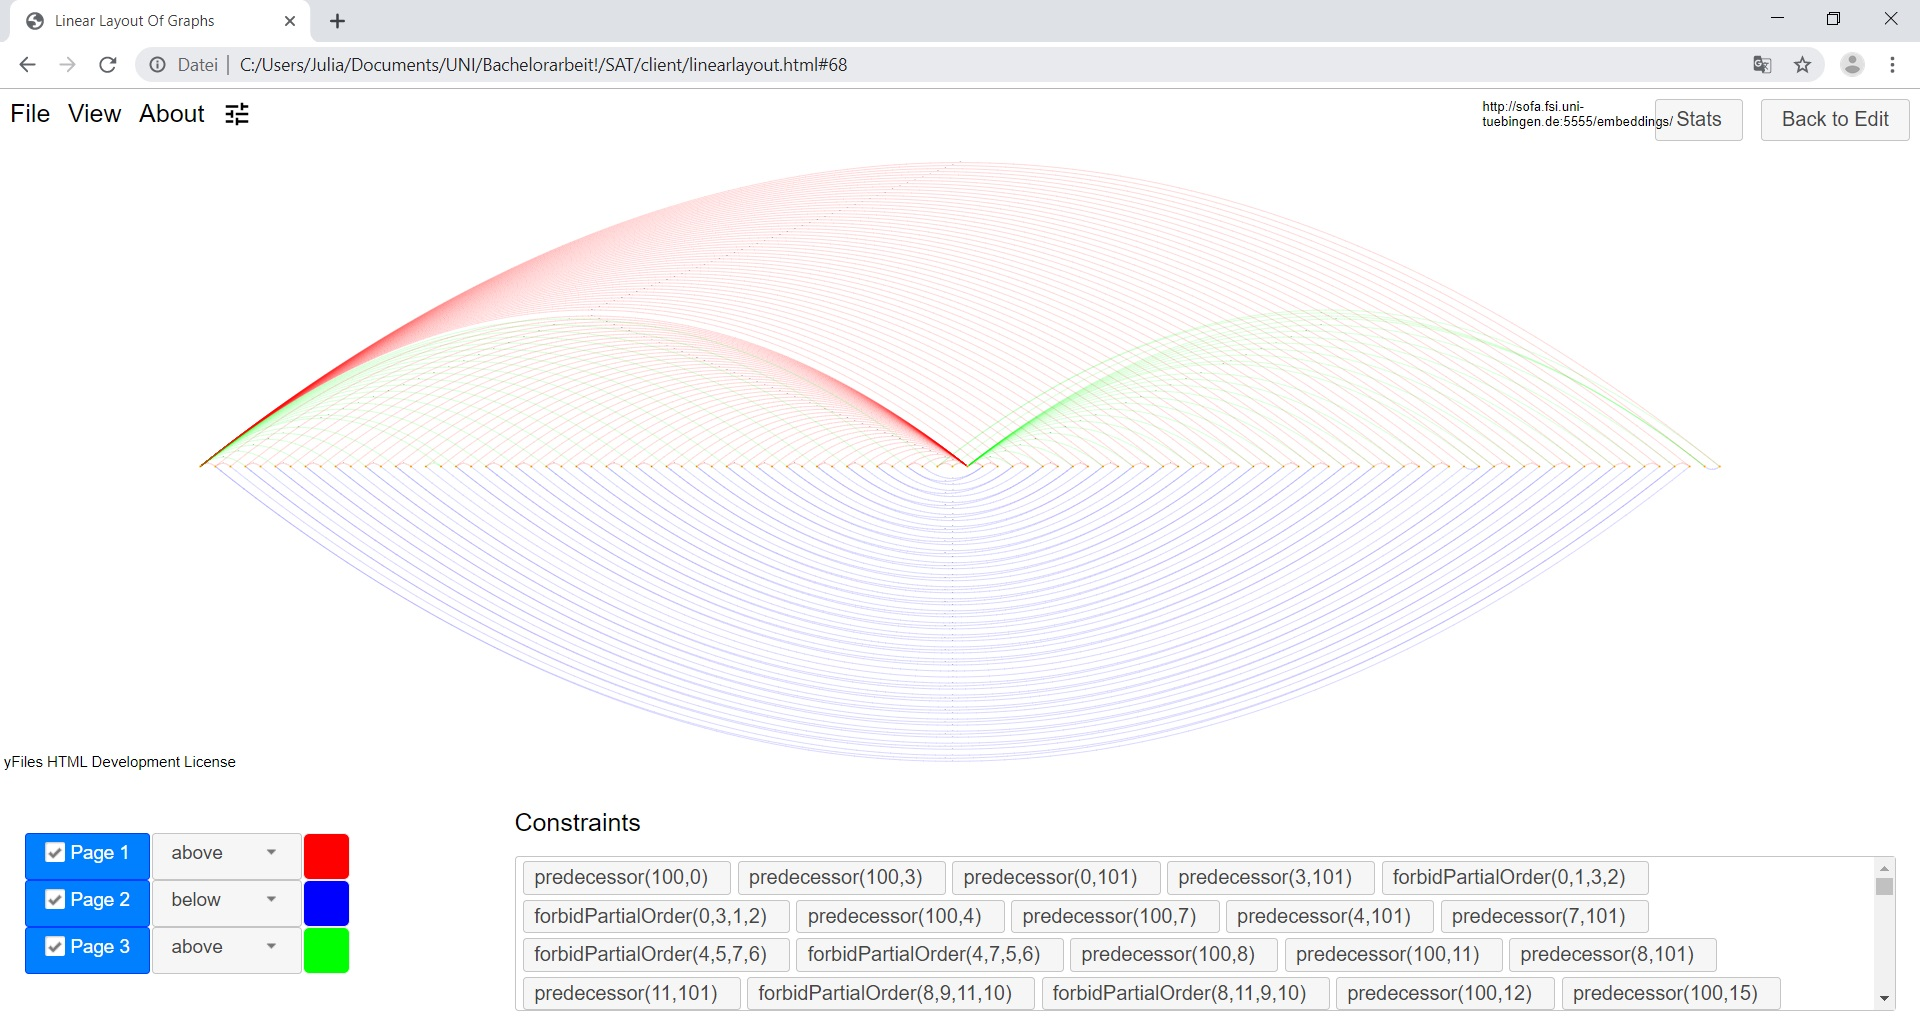
\includegraphics[width=1\textwidth]{figures/stellated-102-274-Solution.jpg}
\caption{The corresponding linear layout to graph in \autoref{s2graph} \label{s2Sol}}
\end{center}
\end{figure}